\recipe{Leah’s De Facto: The tastiest Kale Salad }
\label{recipe:kale_salad}
\makes{4 portions}
\worktime{\SI{25} \minute}
\totaltime{\SI{2} \hour}
\source{Leah}


\begin{ingredients}

  \item For the salad: 
  \item \SI{100}{\gram} kale 
  \item 2 large carrots, grated 
  \item 1 can chickpeas (400g), drained and rinsed 
  \item A handful of sundried tomatoes, chopped 
  \item Parmesan, grated generously
 
\ingroup{For the dressing}
  \item 2 heaped tbsp tahini 
  \item \SI{1}{\teaspoon} mustard (Dijon, if you’re feeling très chic) 
  \item 1 clove garlic, finely chopped or grated 
  \item \SI{1}{\tablespoon} olive oil 
  \item Juice of $1/2$ lemon 
  \item 1 or \SI{2}{\tablespoon} water (to loosen, as needed) 
  \item Pinch of salt + pepper 
\end{ingredients}


\begin{method}

Kale Prep (the secret to a good kale salad). 
Add 100g of the kale to a large bowl. Strip off any tough stalks. . Sprinkle
over 1 teaspoon of salt and massage (oh yeah baby) the kale for 2 minutes
until it softens.

Build the base.
Add all the rest of the ingredients

Make the dressing.
In a small bowl, whisk together all the dressing ingredients. Then add 1–2
tablespoons of water until it reaches a creamy, pourable consistency. 

Combine.
Pour the dressing over the salad and mix. Really get in there. Let
everything get coated. 

Parmesan Finale.
Rain down freshly grated Parmesan. As much as your heart desires 
  
\end{method}

\begin{figure}[h]
  	\centering
  	
	\begin{tikzpicture}
  		% Save the image in a box to get its dimensions
  		\sbox0{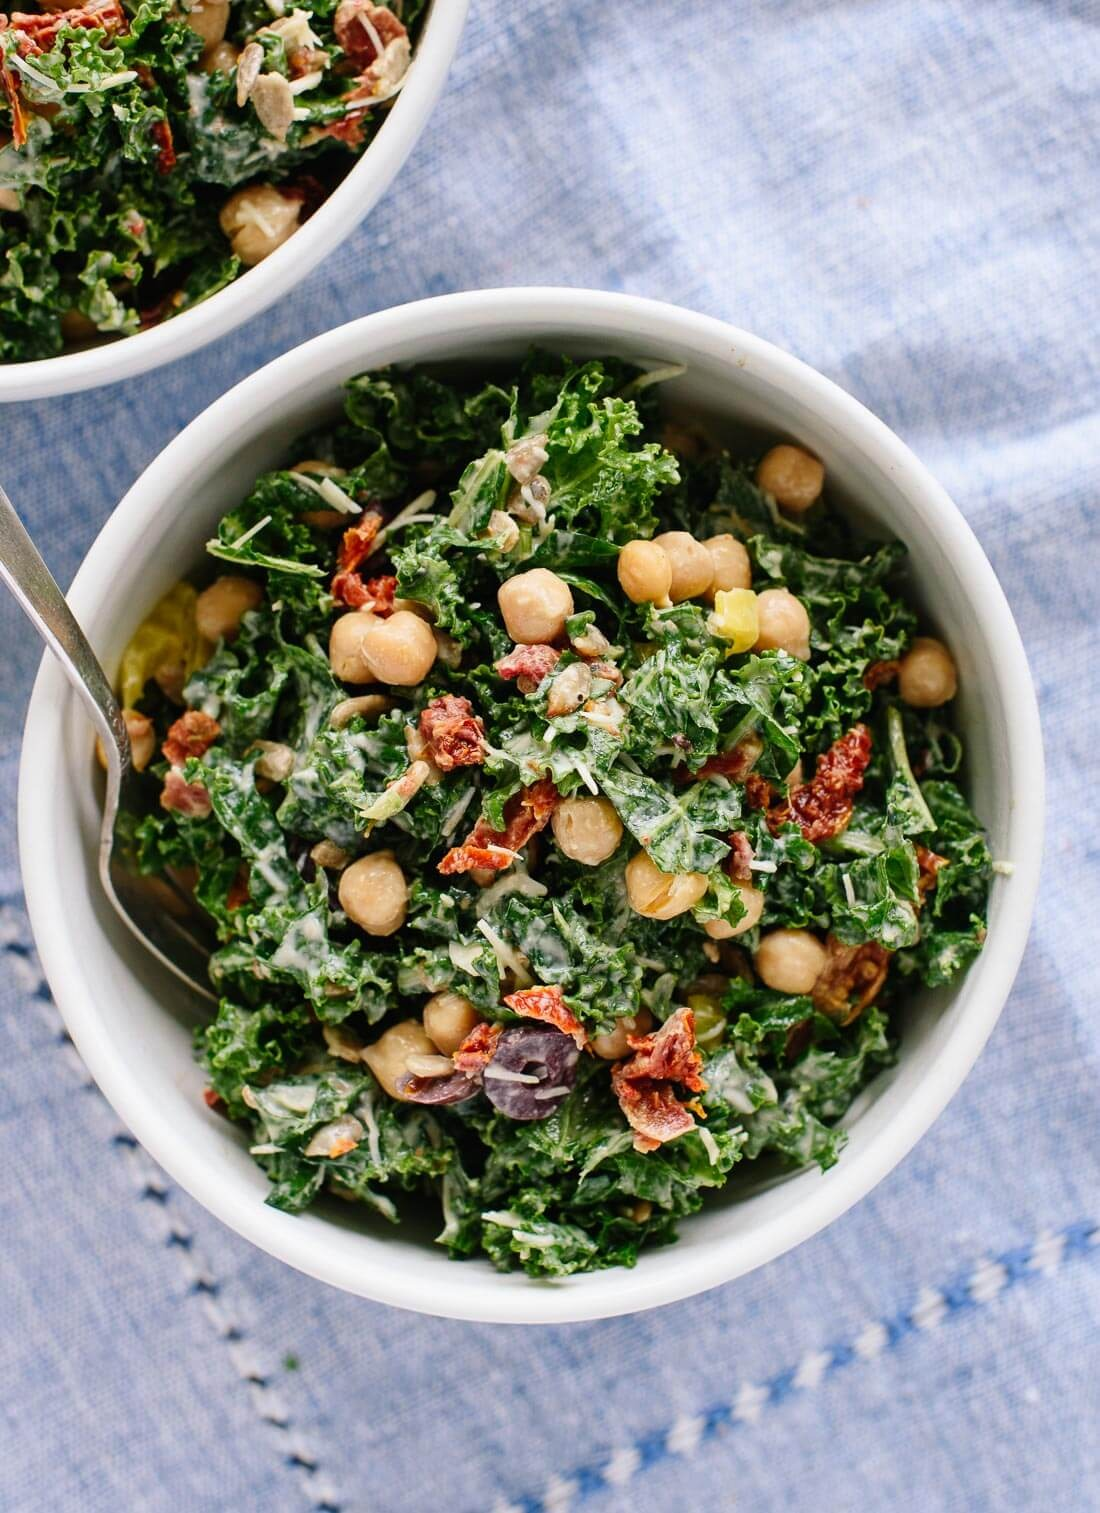
\includegraphics[width = \linewidth]{images/kaleSalad.jpeg}}%
  
  		% Draw a clipping rectangle with rounded corners
  		\path[clip, rounded corners=0.5cm] (0,0) rectangle (\wd0,7cm);
  
  		% Place the image inside the clipped area
  		\node[inner sep=0pt, outer sep=0pt, anchor=south west] at (0, -3cm) {\usebox0};
	\end{tikzpicture}

\end{figure}

\begin{notes}
Enjoy 
You did it!
\end{notes}

